%%
%% This is file `tikzposter-template.tex',
%% generated with the docstrip utility.
%%
%% The original source files were:
%%
%% tikzposter.dtx  (with options: `tikzposter-template.tex')
%% 
%% This is a generated file.
%% 
%% Copyright (C) 2014 by Pascal Richter, Elena Botoeva, Richard Barnard, and Dirk Surmann
%% 
%% This file may be distributed and/or modified under the
%% conditions of the LaTeX Project Public License, either
%% version 2.0 of this license or (at your option) any later
%% version. The latest version of this license is in:
%% 
%% http://www.latex-project.org/lppl.txt
%% 
%% and version 2.0 or later is part of all distributions of
%% LaTeX version 2013/12/01 or later.
%% 
 

\documentclass[a0paper,landscape]{tikzposter} %Options for format can be included here

 % Title, Author, Institute
\title{DocLoop: harvesting reader feedback for Open Educational Resources
%  Channelling reader feedback into Open Educational Resources
 }
\author{Sebastian Nordhoff \& Andreas Pittrich}
\institute{Language Science Press \qquad\qquad  DocLoop  \qquad}
% \titlegraphic{LogoGraphic Inserted Here}
\titlegraphic{~\vspace*{-\baselineskip}}

 %Choose Layout
\usetheme{Default}
\usetikzlibrary{arrows,quotes,positioning}
\usepackage{url}
\newcommand{\pictitle}[1]{
\fbox{\color{black}\Large #1\vphantom{fj}}
}
\newcommand{\arrowlabel}[1]{
\colorbox{white}{\color{black}\Large\bfseries #1\vphantom{fj}}
}
\setlength\fboxsep{10pt}
\begin{document}

 % Title block with title, author, logo, etc.
\maketitle[width=85cm]
\begin{columns} 
\column{0.23}  
\block[titleleft]{Starting point\vphantom{j}}{
Readers can already annotate documents on the web with PaperHive or hypothes.is. But how to get their comments to the original authors in a useful format? 
}
\column{0.45}  
\block[titleleft]{Solution\vphantom{j}}{
 DocLoop closes a gap between annotations on the readers side and todo lists on the author's side. Readers' comments are directly fed into author's issue management tools. These comments can easily be addressed in future versions of the document. Which can then be annotated. And fed into todo lists. And incorporated. Repeat ad lib.
 }
\column{0.32}  
\block[titleleft]{Empowerment}{
 A low-threshold way to leave comments makes it easier for demographic groups less represented in academia to make their voice heard. 
 This is especially impotant for textbooks, which should reflect the diversity of human society. 
 }
 \end{columns}
 \begin{columns} 
\column{0.2}
 %Second column with first block's top edge aligned with with previous column's top.

 % Second column - first block

\block[titleleft]{Domains}{
\begin{itemize}
 \item Open Educational Resources
 \item Open review 
 \item Community proofreading
\end{itemize}
} 

\begin{subcolumns}
    \subcolumn{0.5} \block{Source adapters}{\begin{itemize}\item PaperHive\item (hypothes.is)\end{itemize} }
    \subcolumn{0.5} \block{Target adapters}{\begin{itemize}\item GitHub\item(Trello)\item(Redmine)\item(Wiki)\end{itemize}}
\end{subcolumns}

\block[titleleft]{Technology}{
\begin{itemize}  
 \item  Node.JS
 \item  MongoDB 
 \item \url{https://github.com/docLoop}
 \item GNU General Public License v3.0
\end{itemize}
}

\block[titleleft]{Give it a try!}{
\begin{itemize}
 \item  Leave a comment at \url{https://paperhive.org/documents/remote?type=langsci&id=oldmacdonald}
 \item Check Github issue list at \url{https://github.com/langsci/oldmacdonald/issues}\\
 \parbox{10cm}{\item Use the laptop next to this poster or your own device}~~\parbox{5cm}{\includegraphics[width=4cm]{qrcode.eps}} 
\end{itemize}
}



 % Second column - second block
% \block[titlewidthscale=0.6, bodywidthscale=0.8]
% {Variable width title}{Block with smaller width.}

 % Second column - third block
% \block{}{Block with no title}

 % Second column - A collection of blocks in subcolumn environment.
% \begin{subcolumns}
%     \subcolumn{0.27} \block{1}{First block.} \block{2}{Second block}
%     \subcolumn{0.4} \block{Sub-columns}{Sample subblocks\\Second subcolumn}
%     \subcolumn{0.33} \block{4}{Fourth} \block{}{Final Subcolumn block}
% \end{subcolumns}

 % Bottomblock
\block{}{ 
% Supported by
% 
\includegraphics[width=13mm]{prototypefund.pdf}Prototypefund   
\scriptsize\noindent
The 22nd International Conference on Electronic Publishing.
Connecting the Knowledge Commons: 
From Projects to Sustainable Infrastructure.
June 2018.
University of Toronto
}
 % FIRST column
\column{0.8}% Width set relative to text width

\block{The document cycle}{
\begin{tikzpicture}

\def \n {4}
\def \radius {15cm}
\def \margin {8} % margin in angles, depends on the radius
\def \offset {110} 

\node[draw, rectangle, text width=38cm] (src) at ({90 * (4 - 1) + \offset}:\radius) [xshift=15cm, yshift=2cm] {\pictitle{Editor}\\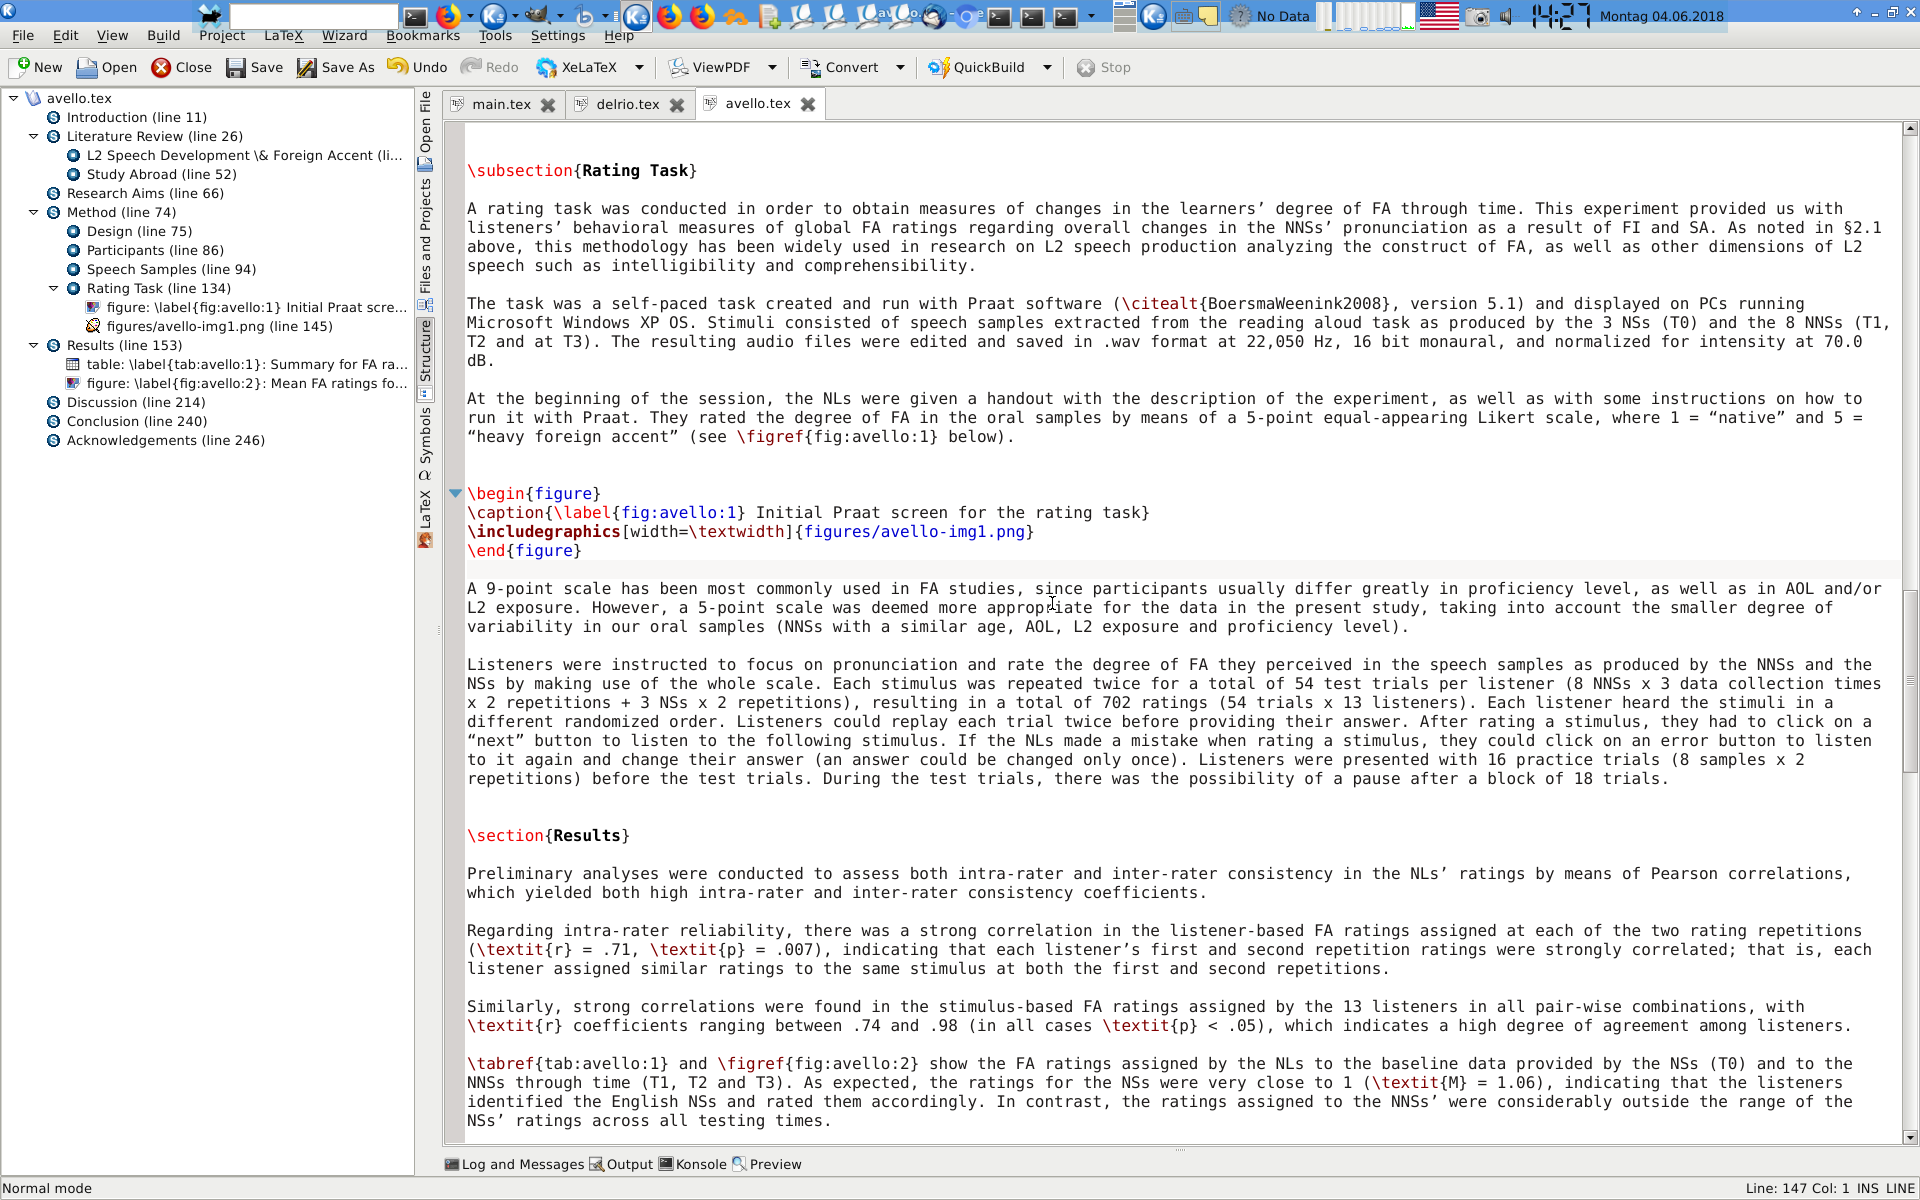
\includegraphics[width=38cm]{src.png}};
\node[draw, rectangle, text width=15cm] (pdf) at ({90 * (3 - 1) + \offset}:\radius) [xshift=10cm]  {\pictitle{Viewer}\\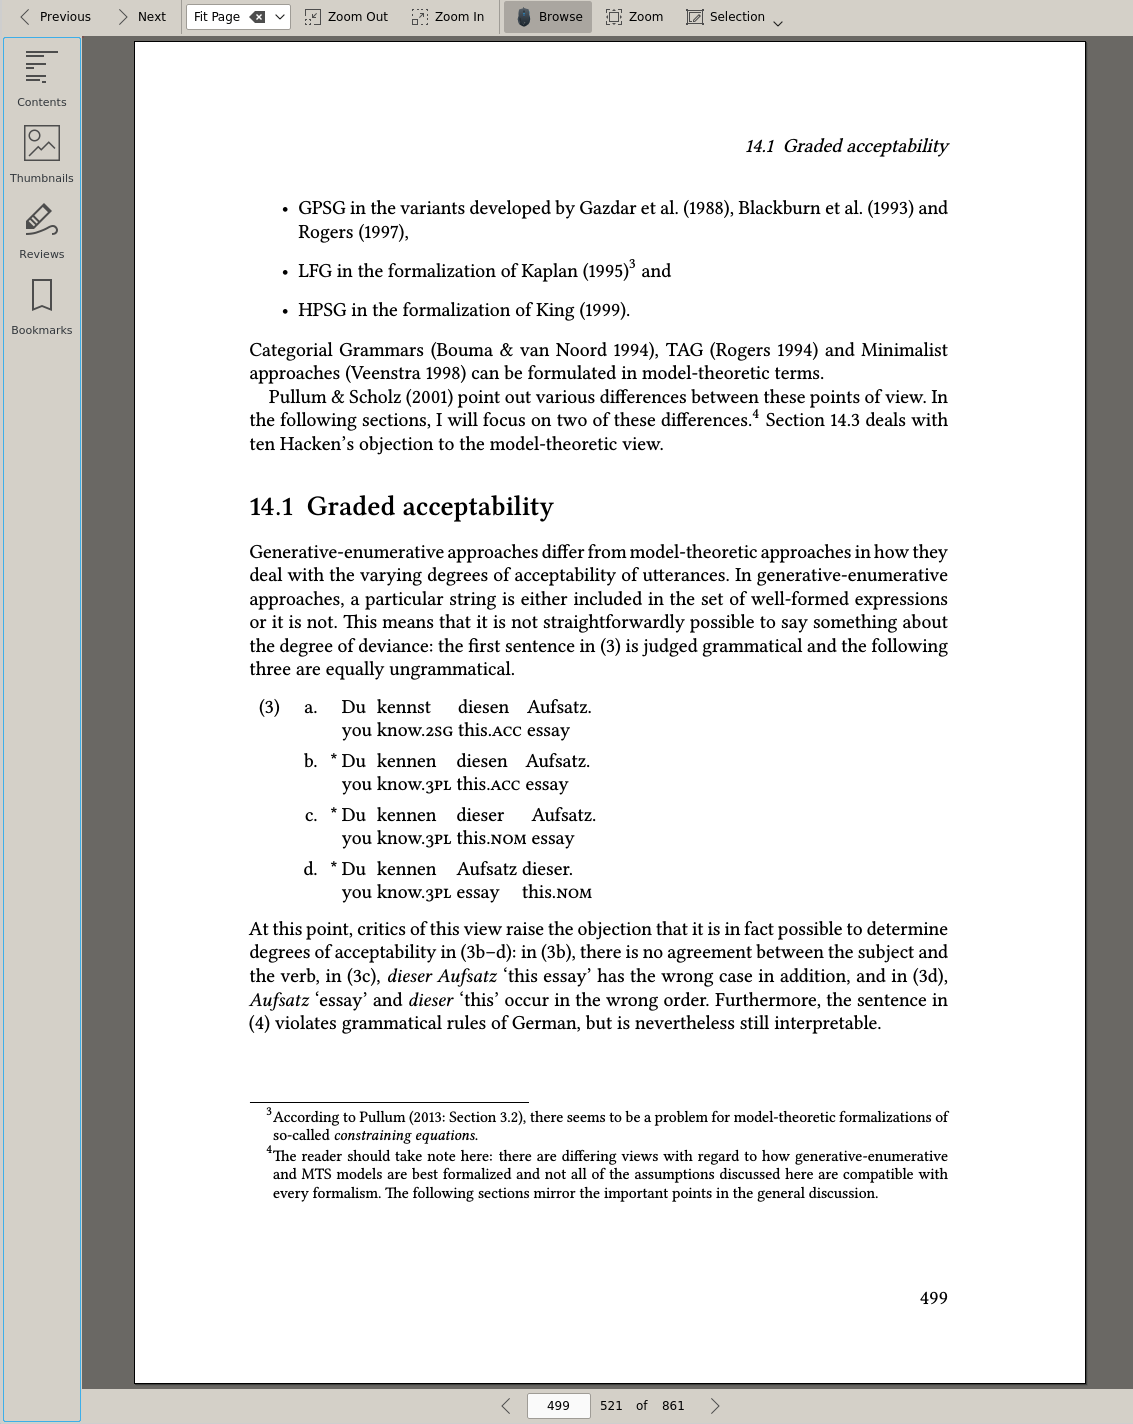
\includegraphics[width=15cm]{pdf.png}};
\node[draw, rectangle, text width=38cm] (ph)  at ({90 * (2 - 1) + \offset}:\radius) {\pictitle{PaperHive}\\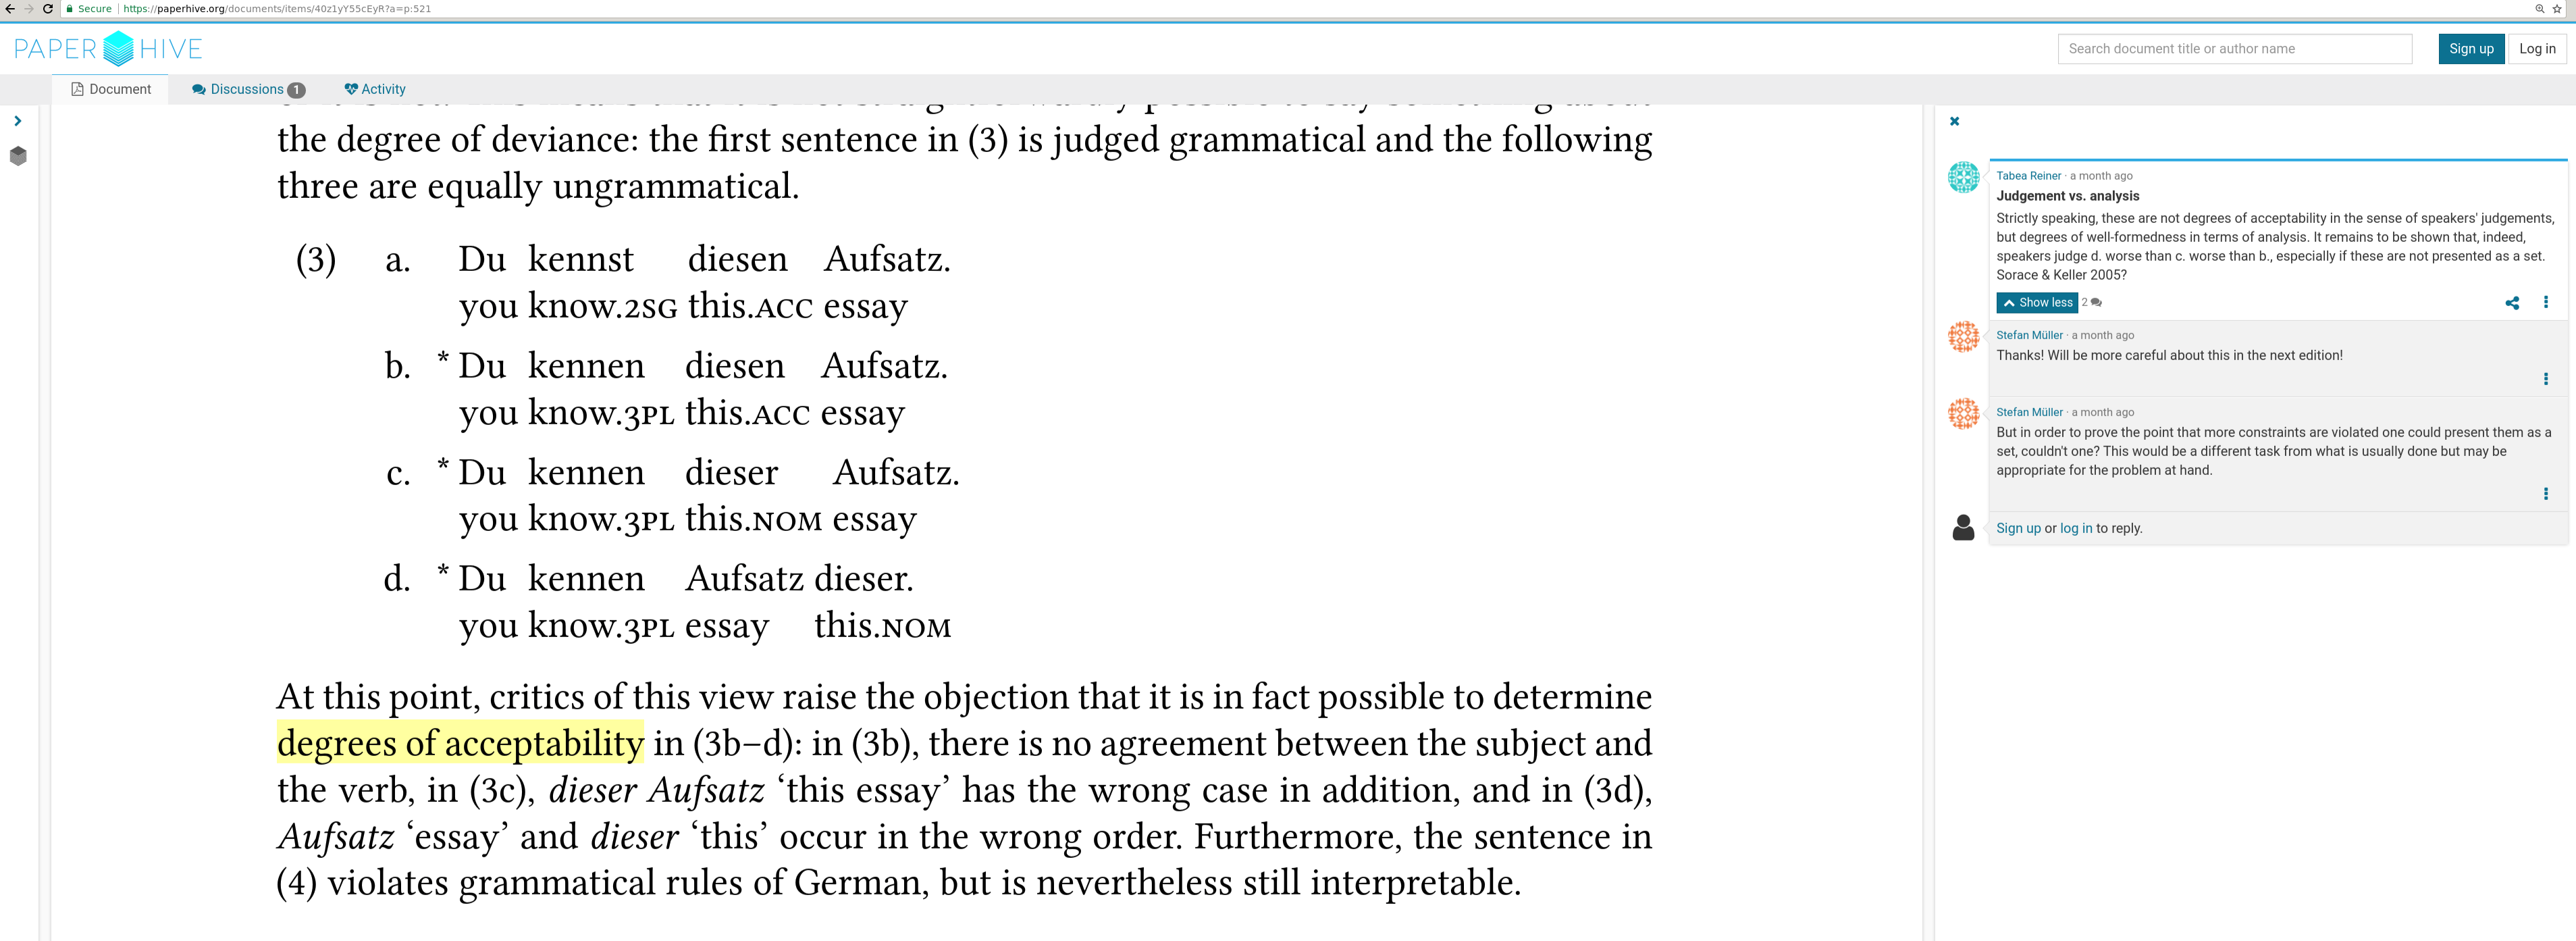
\includegraphics[width=38cm]{paperhive.png}};
\node[draw, rectangle, text width=17cm] (gh)  at ({90 * (1 - 1) + \offset}:\radius) {\pictitle{Issue tracker}\\ 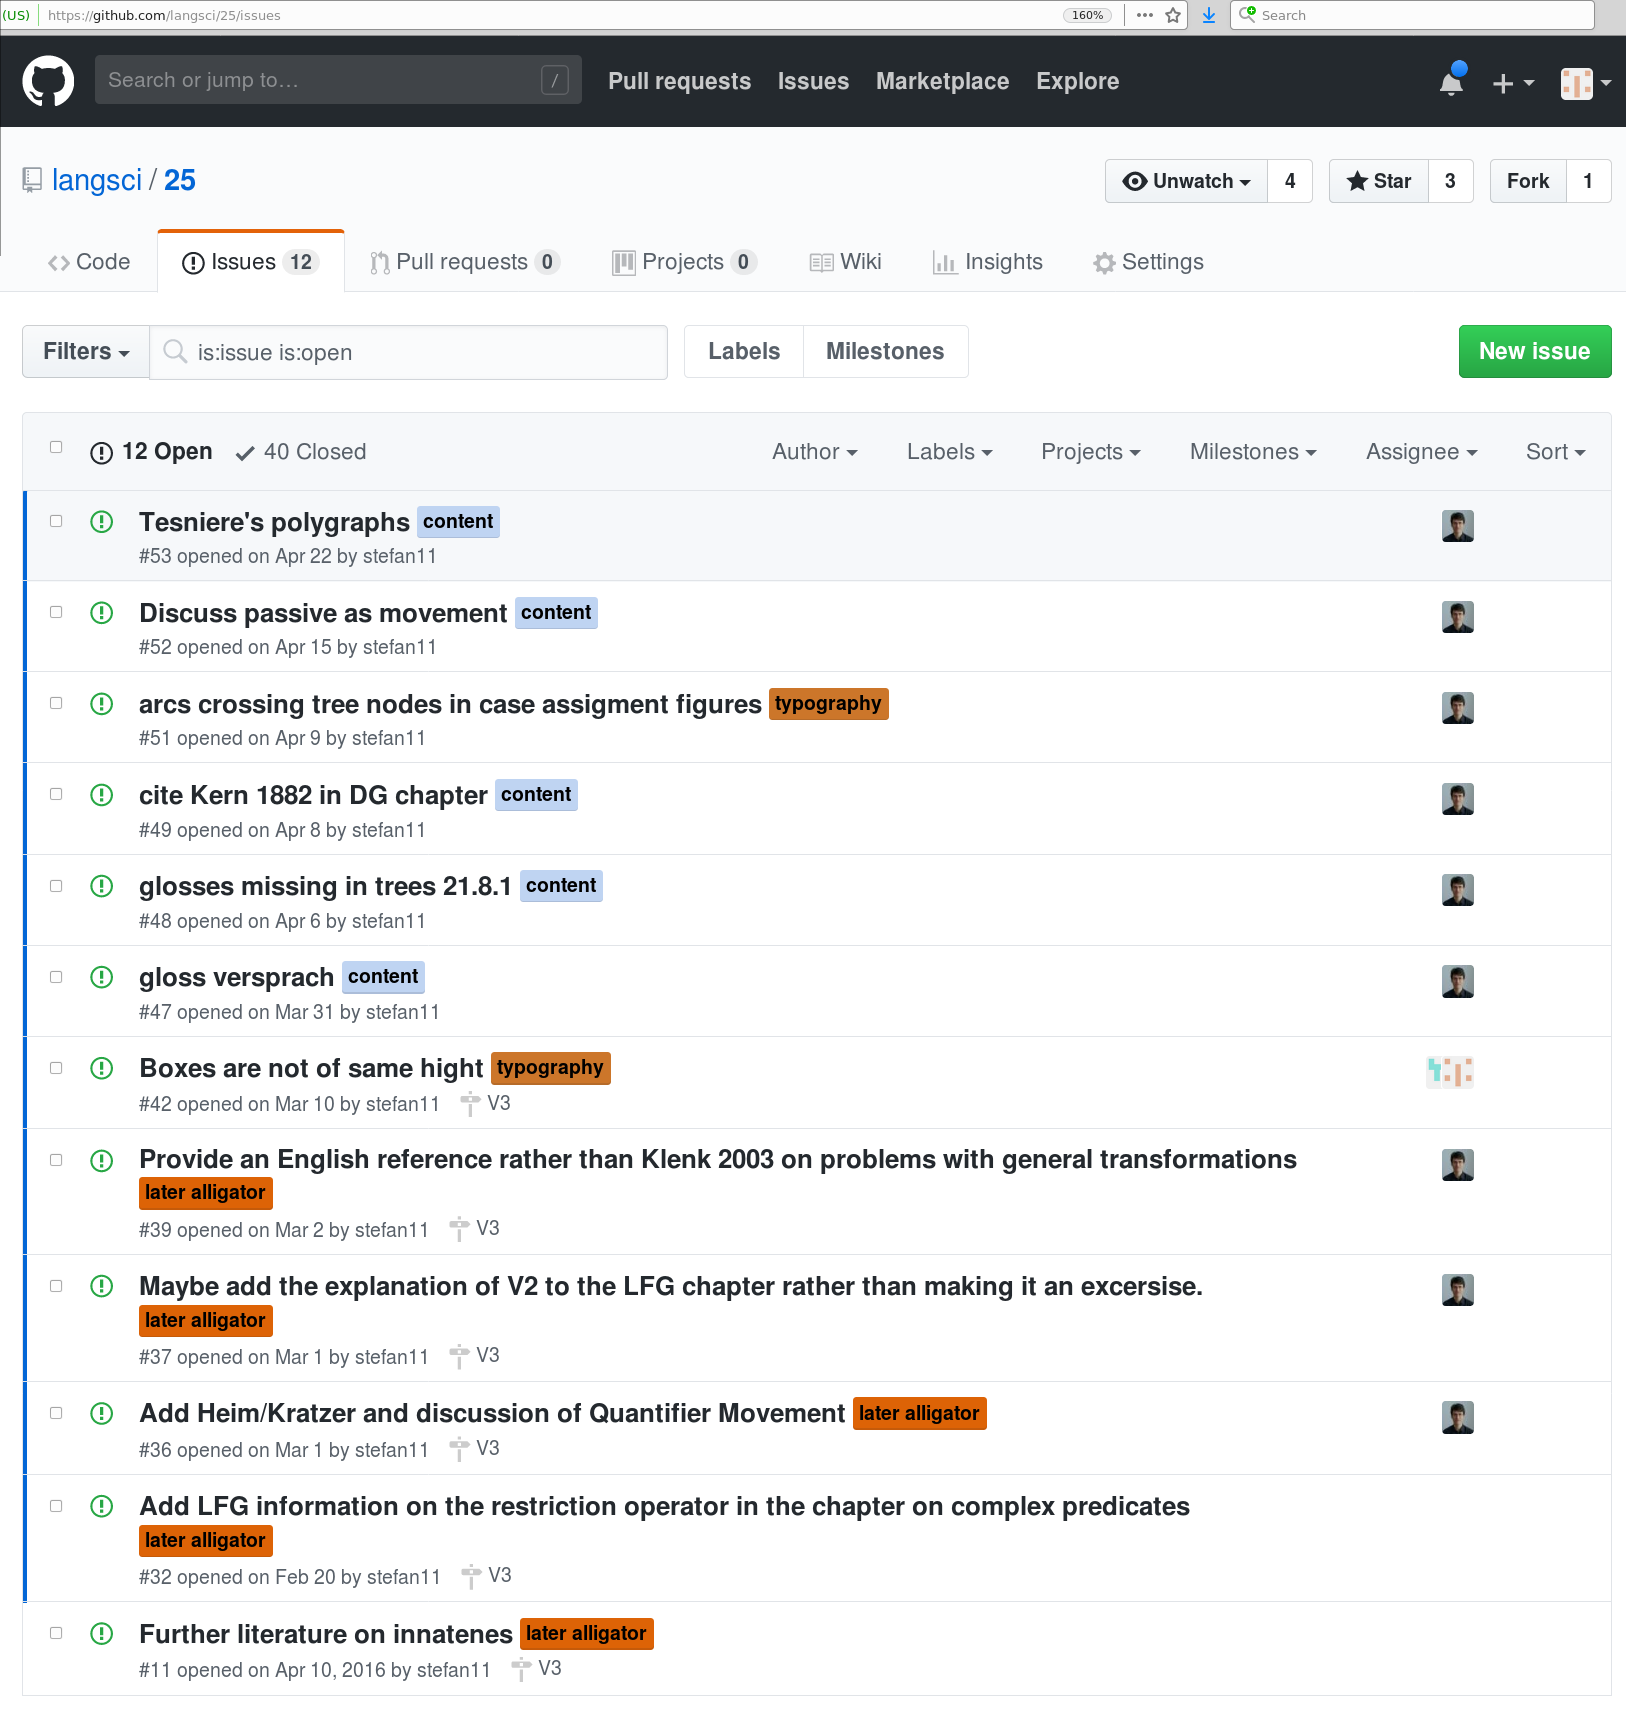
\includegraphics[width=17cm]{github.png}};
  
 
\path[line width=5mm,,lightgray, bend right=20, out=30, in=150,->] (src.south east) edge ["\arrowlabel{generate pdf}"]   (pdf.east) {};  
\path[line width=5mm,,lightgray, bend left=20, out=30, in=130,->] (pdf.south west) edge ["\arrowlabel{send to PaperHive}"]     (ph.south) {};  
\path[line width=5mm, bend right=20, out=30, in=150,->,dash pattern=on 3pt off 12pt, blue] (ph.north west) edge ["\arrowlabel{harvest comments}"]     (gh.west) {};  
\path[line width=5mm,,lightgray, bend right=20, out=30, in=130,->] (gh.north east) edge ["\arrowlabel{address issues}"]     (src.north) {};   

% % \node [right of=src] {test};
\node [left = 6cm of gh,yshift=-6cm] {
\includegraphics[width=5cm]{docloop.pdf}};
\end{tikzpicture}
}
% \note{Note with default behavior}
% \note[targetoffsetx=12cm, targetoffsety=-1cm, angle=20, rotate=25]
% {Note \\ offset and rotated}

%  % First column - second block
% \block{Block titles with enough text will automatically obey spacing requirements }
% {Text\\Text}
% 
%  % First column - third block
% \block{Sample Block 4}{T\\E\\S\\T}
% 

\end{columns}
% \block[titleleft, titleoffsetx=2em, titleoffsety=1em, bodyoffsetx=2em,%
%  bodyoffsety=-2cm, roundedcorners=10, linewidth=0mm, titlewidthscale=0.7,%
%  bodywidthscale=0.9, bodyverticalshift=2cm, titleright]
% {Block outside of Columns}{Along with several options enabled}

\end{document}



\endinput
%%
%% End of file `tikzposter-template.tex'.
